\subsection{Technische Basis}
Umgesetzt wird das Newsboard in Java, sowohl wegen persönlicher Präferenzen der Autoren,
sowie der Tatsache, dass hauptsächlich Java als Programmiersprache
an der FH Bielefeld gelehrt wird. So werden der Weiterentwicklung des Newsboards
durch weitere Studenten keine vermeidbaren Hürden in den Weg gestellt.
Darüber hinaus gibt es für Java eine große Zahl an ausgereiften
und gut dokumentierten Bibliotheken, sowie verlässliche Frameworks zum 
Build-Management.

Als Basis für das Newsboard wird das Spring-Framework im Zusammenspiel mit Maven
als Build-Management-Tool verwendet. Diese Kombination ist in der Praxis bewährt,
ist flexibel für verschiedenste Anwendungsfälle, sowie ohne große Einarbeitungszeit
gut zu benutzen.

Spring bietet außerdem eine sehr ausgereifte Inversion-of-Control, wodurch eine
lose Kopplung der einzelnen Komponenten untereinander gewährt wird\cite{fowler-ioc}.
In der Umsetzung von Spring werden dabei die einzelnen Klassen nur mit
Annotationen versehen und haben ansonsten keine zwingenden Abhängigkeiten
zum Spring Framework.

Darüber hinaus können neben konkreten Klassen auch Abhängigkeiten zu Interfaces
aufgelöst werden, welche wiederum in ihrer Auflösung in konkrete Klassen
durch die Konfiguration von Spring beeinflusst werden können.
So kann zum Beispiel entweder eine Konfiguration für eine SQL-Datenbank,
oder einen anderen Datenspeicher angelegt werden und in Abhängigkeit
der aktivierten Konfiguration werden unterschiedliche Implementierungen injiziert.

\subsection{Datenmodell}
Das Datenmodell des Newsboards wird mit dem relationalen Datenbankmanagementsystem MySQL
abgebildet. Als weitverbreitetes Open-Source Produkt eignet es sich optimal, um im
Newsboard eingesetzt zu werden. Basierend auf dem vom ERD beschriebenen Modell
(Abb. \ref{erd}) des Newsboards wurde ein physisches Modell für MySQL entwickelt
(Abb. \ref{physical_model}).

\begin{figure}[h]
	\centering
	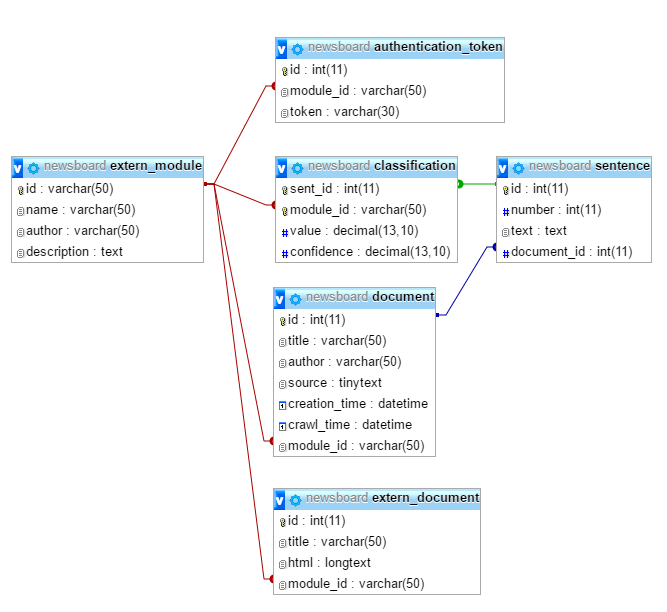
\includegraphics[scale=0.8]{content/physical-model.png}
	\label{physical_model}
	\caption{Physisches Modell des Newsboards}
\end{figure}

Das Modell wird in der Schnittstelle über acht Klassen abgebildet (Abb. \ref{uml_model}).
Hier zeigen sich Abweichungen in der Abbildung der tatsächlichen Tabellen. So ist die
Klasse Document eine Containerklasse, die die Metainformationen und die Sätze des
Dokuments speichert. Um die Metainformationen eines Dokumentes zu struktieren, ist für
sie eine eigene Klasse vorhanden: DocumentMetaData. Für Sätze steht die Klasse Sentences
bereit, die zudem eine Liste mit allen Klassifikationen eines Satzes beinhaltet. Die 
Klasse RawDocument dient rein zum Einlesen von Dokumenten, die von Crawlern bereitgestellt
werden. Sie besteht aus den MetaDaten und dem Text eines Dokumentes. Nach dem Einlesen
wird ein RawDocument in ein Document überführt.

\begin{figure}[h]
	\centering
	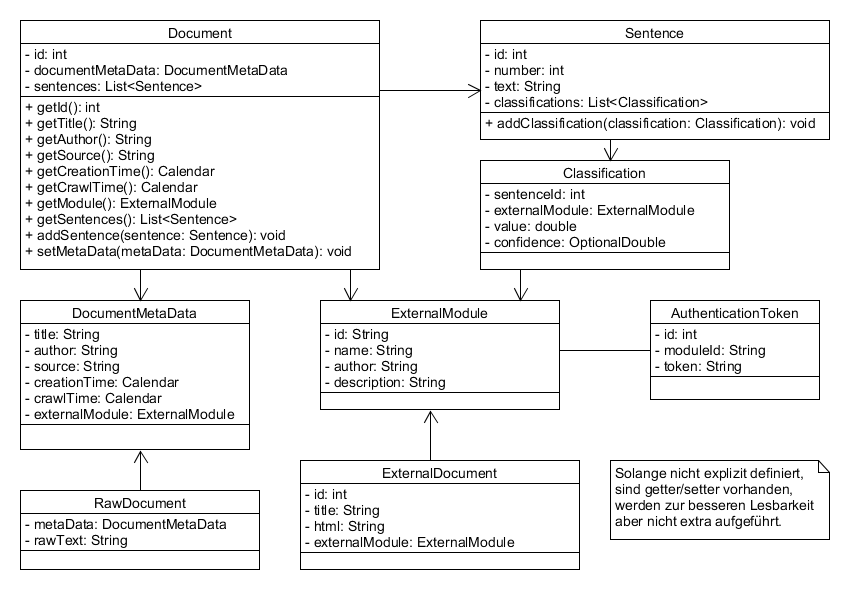
\includegraphics[scale=0.5]{content/uml-model.png}
	\label{uml_model}
	\caption{Diagramm der intern verwendeten Modellklassen}
\end{figure}

Für die Kommunikation zwischen der Schnittstelle und der Datenbank wurde auf das Data-
Access-Object Design Muster gesetzt, um eine hohe Modularität und Flexibilität zu
gewährleisten \cite{dao-pattern}. Beim DAO Muster werden verschiedene Interfaces
verwendet, um den Zugriff auf Datenbankoperationen zu maskieren, während die eigentliche
Übertragungslogik pro Datenquelle eigens entwickelt werden kann. Das, und die
Dependency-Injection-Funktion Springs ermöglicht es, im Falle eines Datenbankwechsels von
MySQL hin zu einem beliebigen anderem System, die Schnittstelle fast ohne Anpassungen
weiter verwenden zu können.

\subsection{Dokumentverarbeitung}
Um die RawDocuments, die die Crawler über die REST-Schnittstelle bereitstellen,
in Document-Objekte zu überführen, muss der Text in einzelne Sätze überführt werden.
Zu diesem Zweck wurde die Klasse RawDocumentProcessor implementiert. Sie nutzt die
Apache openNLP Bibliothek, um den Plaintext von RawDocuments in Sentences zu überführen.

Apache openNLP ist eine Sammlung verschiedener Werkzeuge, um mit Java einfach verschiedene 
NLP-Probleme zu lösen \cite{opennlp}. Es liefert neben verschiedenen 
Machine-Learning-Algorithmen auch fertige Modelle zum Einlesen mit, unter anderem
zum Finden von einzelnen Sätzen. Diese Modelle sind in verschiedenen Sprachen vorhanden,
für das Newsboard wird eines zur Erkennung der deutschen Sprache verwendet.

OpenNLP stellt zur Satzerkennung das Interface SentenceDetector und die davon ableitende
Klasse SentenceDetectorME zur Verfügung. SentenceDetectorME nutzt ein Maximum-Entropy-Modell
zur Klassifizierung von Satzzeichen, die einen Satz beenden. Sie wird auch im
RawDocumentProcessor eingesetzt. Über einen einfachen Methodenaufruf kann so ein kompletter
Text verarbeitet werden, die Kopplung zu openNLP bleibt trotzdem sehr gering, da nur hier
auf die Bibliothek gesetzt wird.

\subsection{Schnittstelle}
Zur Implementierung der REST-Endpoints der Schnittstelle werden die in Spring enthaltenen
Controller-Features genutzt. Um damit einen Endpoint zu bedienen, reicht es aus,
eine Methode innerhalb einer Controller-Klasse mit \texttt{RequestMapping} zu annotieren.
Listing \ref{lst:restExample} zeigt Beispielhaft, wie ein solcher Endpoint unter Angabe der
Annotations-Parameter implementiert werden kann.

Der Rückgabewert der Methode wird so direkt als Antwort an den Client zurückgeliefert.
Darüber hinaus können mit Hilfe der Dependency-Injection von Spring weitere Parameter
definiert werden, die z.B. die HTTP-Anfrage, oder die Antwort wie im Beispiel.
\vspace{1em}

\begin{java}{Implementierung eines REST-Endpoints mit Spring}{lst:restExample}
@RestController
public class RestApiController {
	[...]
	@RequestMapping(path = "/document", method = RequestMethod.GET, produces = MediaType.APPLICATION_XML_VALUE)
	public String listDocuments(HttpServletResponse response) {
		[...]
		return documents;
	}
	[...]
}
\end{java}

\begin{itemize}
	\item \textbf{GET /document}
	Lesen einer Liste aller Dokumente
	\item \textbf{GET /document/\{id\}}
	Lesen eines spezifizierten Dokuments
	\item \textbf{PUT /document}
	Einfügen eines neuen Dokuments durch einen Crawler
	\item \textbf{GET /unclassified}
	Lesen aller Dokumente, die vom aktuellen Classifier noch nicht bewertet wurden
	\item \textbf{PUT /classify}
	Einfügen neuer Klassifizierungen durch einen Classifier
\end{itemize}

Über die REST-Endpoints hinaus ist bei der Schnittstelle noch die Verbeitung der XML-Daten,
sowie das Schema zur Validierung interessant.
Da die zu erwartende Datenmengen im Vorhinein nicht abschätzbar sind,
sollte das Lesen und vor allem das Schreiben der XML-Daten möglichst wenig Speicher
verbrauchen, um eventuelle Engpässe zu vermeiden. Beim Lesen ist eine Validierung
gegen das Schema unbedingt notwendig, da nicht davon ausgegangen werden kann,
dass die ankommenden Daten in jedem Fall valide sind.

Aufgrund der Speicheranforderungen ist ein herkömmlicher DOM-Parser in diesem Projekt
nicht geeignet. Gelesen werden die XML-Daten stattdessen mit einem SAX-Parser.

